\section{OpenCL}

\subsection{Language Overview}

Open Computing Language (OpenCL) is a framework for writing applications
designed to be executed across heterogeneous platforms such as central
processing units (CPUs), graphics processing units (GPUs), and accelerator
devices such as the Intel Phi and Field Programmable Gate Arrays (FPGAs). The
language is an open standard maintained by Khronos Group
\footnote{\url{http://www.khronos.org/opencl}}. OpenCL is based on the C99
standard and can be loosely thought of as a subset of the C99 language with some
additional keywords. The first release of the OpenCL standard (OpenCL 1.0) was
on the 8th of December 2008. There have been two subsequent stable releases of
the standard, OpenCL 1.1 and 1.2, on the 14th of June 2010 and 15th of November
2011 respectively. The version with most hardware support is OpenCL 1.1
\footnote{\url{http://www.khronos.org/registry/cl/specs/opencl-1.1.pdf}} and
this standard forms the basis of all discussion on OpenCL in this report.

OpenCL splits the program code into two sections called `host' and `device'.
Host code runs on the CPU and is written in a traditional language such as C or
C++. The host code executes as normal and makes use of APIs exposed by OpenCL to
define how, and where, OpenCL device code is executed.

OpenCL applications are called kernels. A kernel is a function that executes on
an OpenCL capable device. Given the focus of OpenCL is on parallelism, a kernel
is written from the perspective of a single thread instead of requiring explicit
threading code from more familiar models such as POSIX Threads. An OpenCL work
item is similar to a POSIX Thread with a notable exception that OpenCL has no
traditional stack, any `function' calls are actually in-lined by the compiler.
OpenCL kernels are also compiled at runtime thus the host code, and the compiler
itself, can make device-specific optimisations for optimal performance.

\subsection{Models}

To accommodate the variety of devices OpenCL is designed to work with, a more
abstract Memory Model, and Concurrency and Execution model was designed to allow
the programmer full access to the target devices' capabilities.

\subsubsection{Memory Model}

For a traditional C/C++ application, the application programmer can make use of
the primary memory space of the computer, typically DDR2 or DDR3 RAM. There are
caches on the CPU die however no direct control over their contents is offered.
For CPUs this is not an issue, all modern CPUs support automatic caching.
Problems occur when considering other devices, such as a GPU. GPUs do not
typically have automatic caching thus a programmer must make use of OpenCLs
abstract Memory Model, and hardware vendors must map this model to the physical
hardware. The OpenCL memory model defines four different types of memory, each
of which will be outlined below. A simplified diagrammatic representation of the
memory model is shown in Figure \ref{fig:openCLMemoryModel}.

\begin{description}

\item[Global memory] This memory is accessible by all compute units and is
similar to main memory on a traditional CPU system. All work items are able to
access and update everything stored in this memory. For a GPU this is memory is
mapped to the primary memory of the GPU and is typically 1-4GB in size. When
transferring data between the host and device, this is where the data has to
reside. Global memory is denoted as `\_\_global' in an OpenCL kernel.

\item[Constant memory] Constant memory resides in the same space as global
memory and is used for data which is accessed simultaneously by all work items,
or for variables whose values never change. Constant memory is denoted as
`\_\_constant' in an OpenCL kernel.

\item[Local memory] This is scratch pad memory which is only visible to a single
compute unit on the device (think core of a CPU). Local memory can be split up
into distinct sections if a single compute unit is executing multiple work-
groups simultaneously. Local memory is generally on- chip memory and thus has
faster access time than global memory. Local memory is typically on the order of
tens of kilobytes in size. Use of local memory is either statically declared in
the kernel (e.g `\_\_local float[64] localArray') or dynamically allocated at
runtime by the host since OpenCL kernels do not offer dynamic memory allocation.
Variables in local memory are not what would be called `local' in a traditional
application, local variables are in private memory. Variables in local memory
are shared across a single work group, which can contain multiple work items.

\item[Private memory] This is memory that is unique to an individual work item.
Any local variables and non-pointer kernel arguments are private by default.
These are typically mapped to registers although can be spilled over to higher
latency memories if required.

\end{description}

\begin{figure}
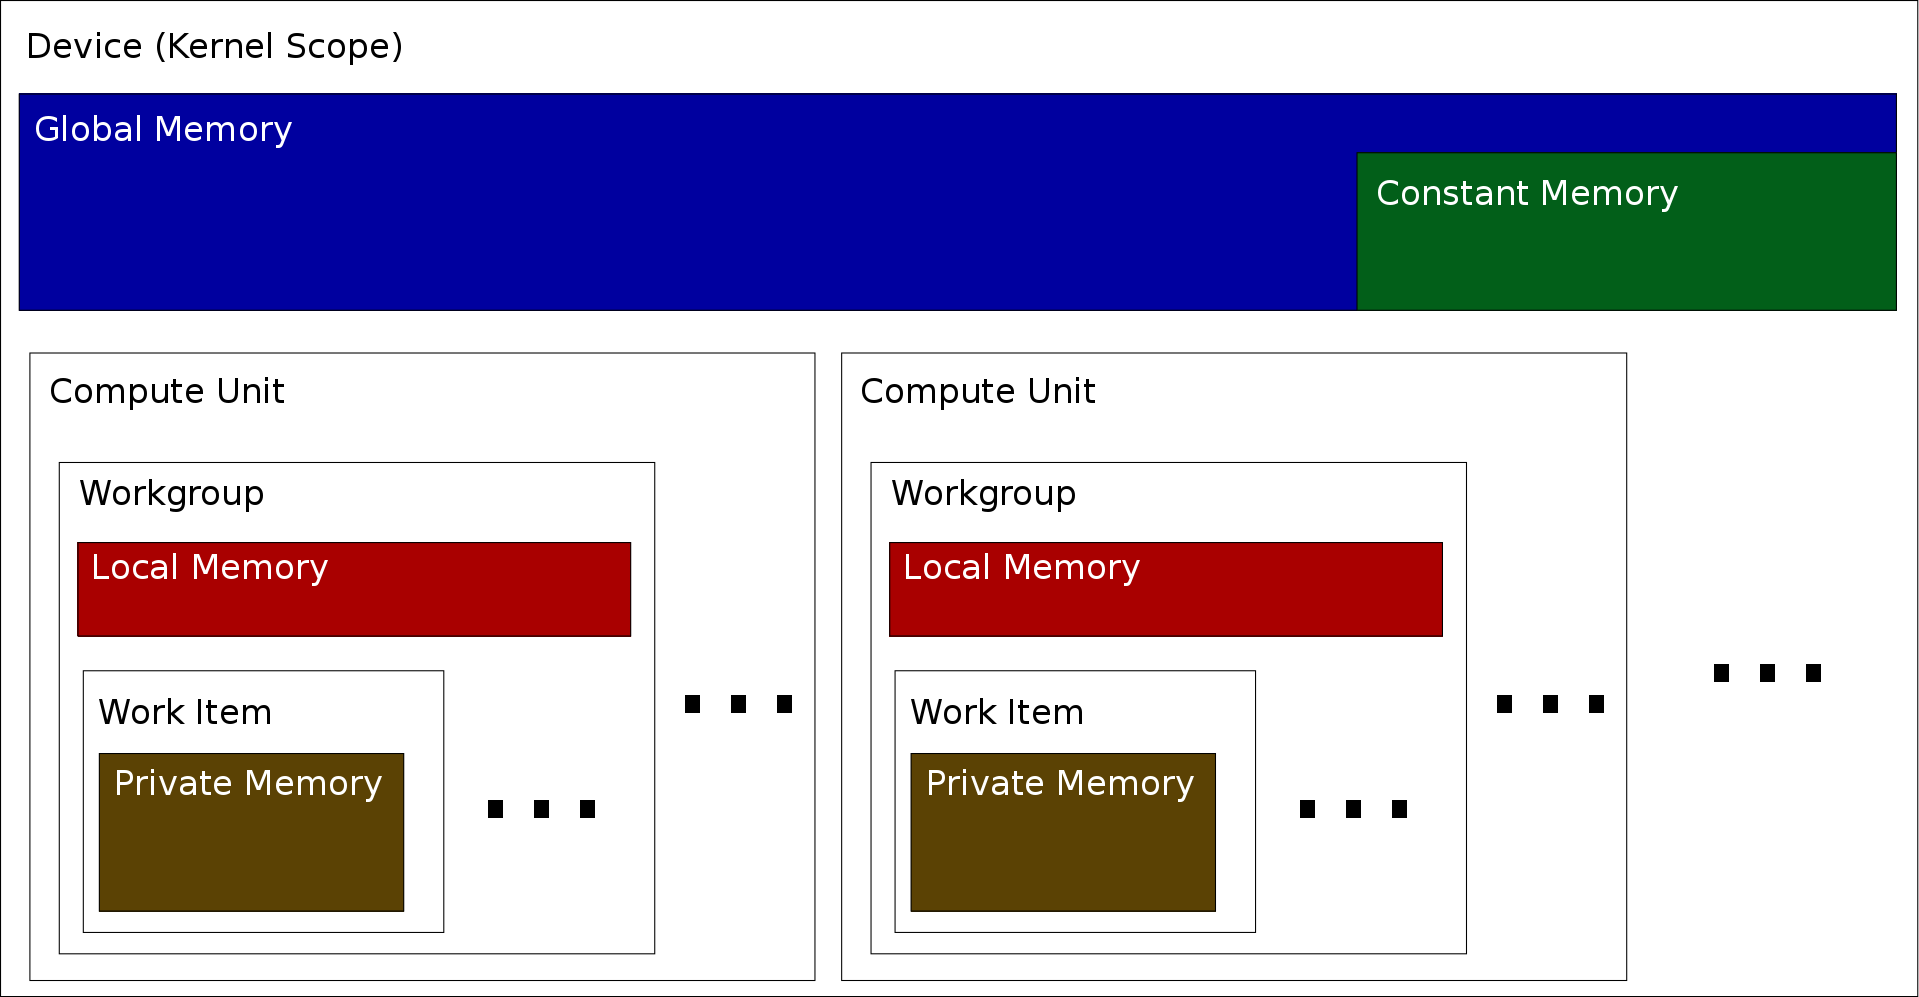
\includegraphics[width=\linewidth]{images/openCLMemoryModel.png}
\caption{Simplified visualisation of OpenCL Memory Model}
\label{fig:openCLMemoryModel}
\end{figure}

\subsubsection{Concurrency and Execution Model}

As shown in Figure \ref{fig:openCLMemoryModel}, OpenCL uses a number of
different terms to describe it's execution model. There is no explicit `thread',
instead OpenCL has work items which are the closest relative to traditional
threads. The OpenCL Concurrency and Execution Model is split into two parts,
host and device, and both will be outlined below.

\paragraph{Host}

\begin{description}

\item[Host program] As discussed previously, a host program is a traditional
program (written in C/C++ for instance) and is executed on a CPU. The host
program is responsible for managing the execution of kernels by creating and
setting up command queues for memory commands, kernel execution commands, and
synchronisation of commands.

\item[Context] The host program defines a context for the kernels. The context
will include the kernels to be executed, the available OpenCL devices, the
program kernels, and the memory objects used by kernels.

\item[NDRange] This stands for N-Dimensional Range and defines how work items
are organised. Work items can be arranged into 1, 2, or 3 dimensions.

\item[Device Type] OpenCL places devices into three different classifications.
CPUs, GPUs, and Accelerators. An example accelerator device would be the Intel
Phi \footnote{\url{http://www.intel.com/content/www/us/en/processors/xeon/xeon-
phi-detail.html}}.

\end{description}

\paragraph{Device}

\begin{description}

\item[Compute Unit] This is a generic term used to describe a multiprocessor on
a GPU, or a core of a CPU. For some devices (such as a GPU) a compute unit will
have dedicated local memory, visible only to itself. A single compute unit can
be assigned multiple work groups.

\item[Kernel] As discussed previously, OpenCL code which runs on an OpenCL
device is known as a kernel. These are written from the perspective of a single
work item (thread).

\item[Work group] This is a collection of work items. An entire work group is
assigned to one compute unit. These work items can share local memory and can
synchronise with one another.

\item[Work item] This closely resembles a single thread. Each work item is
assigned a work group. Every work item can access local memory of its work
group and can access all global and constant memory. A work item will also
have private variables which may or may not fit inside private memory.

\item[Global size] This represents the total number of work items in each
dimension. The multiplication of the global size in each dimension is the total
number of work items being executed for the corresponding kernel.

\item[Local size] This represents the total number of work items in each
dimension for a single work group. The global size for a dimension has to be an
integer multiple of the local size for that dimension for the work group size
to be valid. This is to ensure work groups can fit inside the global dimension
size evenly.

\end{description}

Just as with the Memory Model, different devices will realise the Concurrency
and Execution model differently. These differences will be discussed in the next
section.

\section{Device comparisons}

There are numerous important architecture differences between different classes
of device,

\subsection{CPU and GPU}

\subsection{Intel Phi}

\section{Document Classification}

\subsection{Bloom Filters}

\subsection{Hashed Profile}

% linear probing, hence 4 terms looked at.
